\documentclass[letterpaper]{article}
\usepackage[margin=0in]{geometry}
\pdfmapfile{+cm.map}
\usepackage{type1cm}
\usepackage{tikz}
\pagestyle{empty}
\setlength{\parindent}{0pt}
\hyphenpenalty=10000
\exhyphenpenalty=10000
\begin{document}
\begin{tikzpicture}[remember picture,overlay,x=1in,y=-1in]
\begin{scope}[shift={(current page.north west)}]
\node[anchor=north west,inner sep=0pt,text width=7.4in,align=left,font=\sffamily\fontsize{10.8}{13.50}\selectfont] at (0.55,0.36) {\bfseries Week 14 / Polygon triangulations and flips / Grades 4--5};
\node[anchor=north west,inner sep=0pt,text width=7.2in,align=left,font=\sffamily\fontsize{12.3}{15.38}\selectfont] at (0.65,0.91) {Fill the whole polygon with triangles, using straight lines between printed corners. Lines inside a polygon may meet at corners but may not cross. Keep the corner labels fixed, even if you turn the page. Use tracing paper to change printed lines.};
\node[anchor=north west,inner sep=0pt,text width=7.2in,align=left,font=\sffamily\fontsize{13.4}{16.75}\selectfont] at (0.65,1.78) {\textbf{Problem 1:} Find every filling of the five-corner polygon. Explain how your collection shows that none are missing.};
\begin{scope}
% polygon: regular n=5
\coordinate (v0) at (4.2500,2.9250);
\coordinate (v1) at (6.0112,4.2046);
\coordinate (v2) at (5.3385,6.2750);
\coordinate (v3) at (3.1615,6.2750);
\coordinate (v4) at (2.4888,4.2046);
\draw[line width=0.95pt,line join=round] (v0) -- (v1) -- (v2) -- (v3) -- (v4) -- cycle;
\fill (v0) circle[radius=0.022in];
\node[inner sep=0pt,font=\sffamily\fontsize{13}{14}\selectfont] at (4.2500,2.7350) {A};
\fill (v1) circle[radius=0.022in];
\node[inner sep=0pt,font=\sffamily\fontsize{13}{14}\selectfont] at (6.1966,4.1630) {B};
\fill (v2) circle[radius=0.022in];
\node[inner sep=0pt,font=\sffamily\fontsize{13}{14}\selectfont] at (5.4420,6.4343) {C};
\fill (v3) circle[radius=0.022in];
\node[inner sep=0pt,font=\sffamily\fontsize{13}{14}\selectfont] at (3.0580,6.4343) {D};
\fill (v4) circle[radius=0.022in];
\node[inner sep=0pt,font=\sffamily\fontsize{13}{14}\selectfont] at (2.3034,4.1630) {E};
\end{scope}
\begin{scope}
% polygon: regular n=5
\coordinate (v0) at (1.3500,7.3900);
\coordinate (v1) at (1.8337,7.7414);
\coordinate (v2) at (1.6489,8.3100);
\coordinate (v3) at (1.0511,8.3100);
\coordinate (v4) at (0.8663,7.7414);
\draw[line width=0.95pt,line join=round] (v0) -- (v1) -- (v2) -- (v3) -- (v4) -- cycle;
\fill (v0) circle[radius=0.014in];
\node[inner sep=0pt,font=\sffamily\fontsize{8}{14}\selectfont] at (1.3500,7.2700) {A};
\fill (v1) circle[radius=0.014in];
\node[inner sep=0pt,font=\sffamily\fontsize{8}{14}\selectfont] at (1.9508,7.7151) {B};
\fill (v2) circle[radius=0.014in];
\node[inner sep=0pt,font=\sffamily\fontsize{8}{14}\selectfont] at (1.7143,8.4106) {C};
\fill (v3) circle[radius=0.014in];
\node[inner sep=0pt,font=\sffamily\fontsize{8}{14}\selectfont] at (0.9857,8.4106) {D};
\fill (v4) circle[radius=0.014in];
\node[inner sep=0pt,font=\sffamily\fontsize{8}{14}\selectfont] at (0.7492,7.7151) {E};
\end{scope}
\begin{scope}
% polygon: regular n=5
\coordinate (v0) at (3.2800,7.3900);
\coordinate (v1) at (3.7637,7.7414);
\coordinate (v2) at (3.5789,8.3100);
\coordinate (v3) at (2.9811,8.3100);
\coordinate (v4) at (2.7963,7.7414);
\draw[line width=0.95pt,line join=round] (v0) -- (v1) -- (v2) -- (v3) -- (v4) -- cycle;
\fill (v0) circle[radius=0.014in];
\node[inner sep=0pt,font=\sffamily\fontsize{8}{14}\selectfont] at (3.2800,7.2700) {A};
\fill (v1) circle[radius=0.014in];
\node[inner sep=0pt,font=\sffamily\fontsize{8}{14}\selectfont] at (3.8808,7.7151) {B};
\fill (v2) circle[radius=0.014in];
\node[inner sep=0pt,font=\sffamily\fontsize{8}{14}\selectfont] at (3.6443,8.4106) {C};
\fill (v3) circle[radius=0.014in];
\node[inner sep=0pt,font=\sffamily\fontsize{8}{14}\selectfont] at (2.9157,8.4106) {D};
\fill (v4) circle[radius=0.014in];
\node[inner sep=0pt,font=\sffamily\fontsize{8}{14}\selectfont] at (2.6792,7.7151) {E};
\end{scope}
\begin{scope}
% polygon: regular n=5
\coordinate (v0) at (5.2200,7.3900);
\coordinate (v1) at (5.7037,7.7414);
\coordinate (v2) at (5.5189,8.3100);
\coordinate (v3) at (4.9211,8.3100);
\coordinate (v4) at (4.7363,7.7414);
\draw[line width=0.95pt,line join=round] (v0) -- (v1) -- (v2) -- (v3) -- (v4) -- cycle;
\fill (v0) circle[radius=0.014in];
\node[inner sep=0pt,font=\sffamily\fontsize{8}{14}\selectfont] at (5.2200,7.2700) {A};
\fill (v1) circle[radius=0.014in];
\node[inner sep=0pt,font=\sffamily\fontsize{8}{14}\selectfont] at (5.8208,7.7151) {B};
\fill (v2) circle[radius=0.014in];
\node[inner sep=0pt,font=\sffamily\fontsize{8}{14}\selectfont] at (5.5843,8.4106) {C};
\fill (v3) circle[radius=0.014in];
\node[inner sep=0pt,font=\sffamily\fontsize{8}{14}\selectfont] at (4.8557,8.4106) {D};
\fill (v4) circle[radius=0.014in];
\node[inner sep=0pt,font=\sffamily\fontsize{8}{14}\selectfont] at (4.6192,7.7151) {E};
\end{scope}
\begin{scope}
% polygon: regular n=5
\coordinate (v0) at (7.1500,7.3900);
\coordinate (v1) at (7.6337,7.7414);
\coordinate (v2) at (7.4489,8.3100);
\coordinate (v3) at (6.8511,8.3100);
\coordinate (v4) at (6.6663,7.7414);
\draw[line width=0.95pt,line join=round] (v0) -- (v1) -- (v2) -- (v3) -- (v4) -- cycle;
\fill (v0) circle[radius=0.014in];
\node[inner sep=0pt,font=\sffamily\fontsize{8}{14}\selectfont] at (7.1500,7.2700) {A};
\fill (v1) circle[radius=0.014in];
\node[inner sep=0pt,font=\sffamily\fontsize{8}{14}\selectfont] at (7.7508,7.7151) {B};
\fill (v2) circle[radius=0.014in];
\node[inner sep=0pt,font=\sffamily\fontsize{8}{14}\selectfont] at (7.5143,8.4106) {C};
\fill (v3) circle[radius=0.014in];
\node[inner sep=0pt,font=\sffamily\fontsize{8}{14}\selectfont] at (6.7857,8.4106) {D};
\fill (v4) circle[radius=0.014in];
\node[inner sep=0pt,font=\sffamily\fontsize{8}{14}\selectfont] at (6.5492,7.7151) {E};
\end{scope}
\begin{scope}
% polygon: regular n=5
\coordinate (v0) at (1.3500,8.8900);
\coordinate (v1) at (1.8337,9.2414);
\coordinate (v2) at (1.6489,9.8100);
\coordinate (v3) at (1.0511,9.8100);
\coordinate (v4) at (0.8663,9.2414);
\draw[line width=0.95pt,line join=round] (v0) -- (v1) -- (v2) -- (v3) -- (v4) -- cycle;
\fill (v0) circle[radius=0.014in];
\node[inner sep=0pt,font=\sffamily\fontsize{8}{14}\selectfont] at (1.3500,8.7700) {A};
\fill (v1) circle[radius=0.014in];
\node[inner sep=0pt,font=\sffamily\fontsize{8}{14}\selectfont] at (1.9508,9.2151) {B};
\fill (v2) circle[radius=0.014in];
\node[inner sep=0pt,font=\sffamily\fontsize{8}{14}\selectfont] at (1.7143,9.9106) {C};
\fill (v3) circle[radius=0.014in];
\node[inner sep=0pt,font=\sffamily\fontsize{8}{14}\selectfont] at (0.9857,9.9106) {D};
\fill (v4) circle[radius=0.014in];
\node[inner sep=0pt,font=\sffamily\fontsize{8}{14}\selectfont] at (0.7492,9.2151) {E};
\end{scope}
\begin{scope}
% polygon: regular n=5
\coordinate (v0) at (3.2800,8.8900);
\coordinate (v1) at (3.7637,9.2414);
\coordinate (v2) at (3.5789,9.8100);
\coordinate (v3) at (2.9811,9.8100);
\coordinate (v4) at (2.7963,9.2414);
\draw[line width=0.95pt,line join=round] (v0) -- (v1) -- (v2) -- (v3) -- (v4) -- cycle;
\fill (v0) circle[radius=0.014in];
\node[inner sep=0pt,font=\sffamily\fontsize{8}{14}\selectfont] at (3.2800,8.7700) {A};
\fill (v1) circle[radius=0.014in];
\node[inner sep=0pt,font=\sffamily\fontsize{8}{14}\selectfont] at (3.8808,9.2151) {B};
\fill (v2) circle[radius=0.014in];
\node[inner sep=0pt,font=\sffamily\fontsize{8}{14}\selectfont] at (3.6443,9.9106) {C};
\fill (v3) circle[radius=0.014in];
\node[inner sep=0pt,font=\sffamily\fontsize{8}{14}\selectfont] at (2.9157,9.9106) {D};
\fill (v4) circle[radius=0.014in];
\node[inner sep=0pt,font=\sffamily\fontsize{8}{14}\selectfont] at (2.6792,9.2151) {E};
\end{scope}
\begin{scope}
% polygon: regular n=5
\coordinate (v0) at (5.2200,8.8900);
\coordinate (v1) at (5.7037,9.2414);
\coordinate (v2) at (5.5189,9.8100);
\coordinate (v3) at (4.9211,9.8100);
\coordinate (v4) at (4.7363,9.2414);
\draw[line width=0.95pt,line join=round] (v0) -- (v1) -- (v2) -- (v3) -- (v4) -- cycle;
\fill (v0) circle[radius=0.014in];
\node[inner sep=0pt,font=\sffamily\fontsize{8}{14}\selectfont] at (5.2200,8.7700) {A};
\fill (v1) circle[radius=0.014in];
\node[inner sep=0pt,font=\sffamily\fontsize{8}{14}\selectfont] at (5.8208,9.2151) {B};
\fill (v2) circle[radius=0.014in];
\node[inner sep=0pt,font=\sffamily\fontsize{8}{14}\selectfont] at (5.5843,9.9106) {C};
\fill (v3) circle[radius=0.014in];
\node[inner sep=0pt,font=\sffamily\fontsize{8}{14}\selectfont] at (4.8557,9.9106) {D};
\fill (v4) circle[radius=0.014in];
\node[inner sep=0pt,font=\sffamily\fontsize{8}{14}\selectfont] at (4.6192,9.2151) {E};
\end{scope}
\begin{scope}
% polygon: regular n=5
\coordinate (v0) at (7.1500,8.8900);
\coordinate (v1) at (7.6337,9.2414);
\coordinate (v2) at (7.4489,9.8100);
\coordinate (v3) at (6.8511,9.8100);
\coordinate (v4) at (6.6663,9.2414);
\draw[line width=0.95pt,line join=round] (v0) -- (v1) -- (v2) -- (v3) -- (v4) -- cycle;
\fill (v0) circle[radius=0.014in];
\node[inner sep=0pt,font=\sffamily\fontsize{8}{14}\selectfont] at (7.1500,8.7700) {A};
\fill (v1) circle[radius=0.014in];
\node[inner sep=0pt,font=\sffamily\fontsize{8}{14}\selectfont] at (7.7508,9.2151) {B};
\fill (v2) circle[radius=0.014in];
\node[inner sep=0pt,font=\sffamily\fontsize{8}{14}\selectfont] at (7.5143,9.9106) {C};
\fill (v3) circle[radius=0.014in];
\node[inner sep=0pt,font=\sffamily\fontsize{8}{14}\selectfont] at (6.7857,9.9106) {D};
\fill (v4) circle[radius=0.014in];
\node[inner sep=0pt,font=\sffamily\fontsize{8}{14}\selectfont] at (6.5492,9.2151) {E};
\end{scope}
\node[anchor=north west,inner sep=0pt,text width=6.9in,align=left,font=\sffamily\fontsize{9}{11.25}\selectfont] at (0.55,10.48) {Bellingham Math Circle / Week 14 / F14-45-v2};
\node[anchor=north west,inner sep=0pt,text width=0.36in,align=left,font=\sffamily\fontsize{9}{11.25}\selectfont] at (7.56,10.48) {1};
\end{scope}
\end{tikzpicture}
\null
\newpage
\begin{tikzpicture}[remember picture,overlay,x=1in,y=-1in]
\begin{scope}[shift={(current page.north west)}]
\node[anchor=north west,inner sep=0pt,text width=7.4in,align=left,font=\sffamily\fontsize{10.8}{13.50}\selectfont] at (0.55,0.36) {\bfseries Week 14 / Polygon triangulations and flips / Grades 4--5};
\node[anchor=north west,inner sep=0pt,text width=7.2in,align=left,font=\sffamily\fontsize{13.4}{16.75}\selectfont] at (0.65,0.91) {\textbf{Problem 2:} Erase one inside line and replace it with a different line so the polygon stays filled with triangles. Find every result of one such change from each drawing.};
\begin{scope}
% polygon: regular n=6
\coordinate (v0) at (2.3500,2.0250);
\coordinate (v1) at (3.8439,2.8875);
\coordinate (v2) at (3.8439,4.6125);
\coordinate (v3) at (2.3500,5.4750);
\coordinate (v4) at (0.8561,4.6125);
\coordinate (v5) at (0.8561,2.8875);
\draw[line width=0.95pt,line join=round] (v0) -- (v1) -- (v2) -- (v3) -- (v4) -- (v5) -- cycle;
\draw[line width=0.85pt] (v0) -- (v2);
\draw[line width=0.85pt] (v0) -- (v3);
\draw[line width=0.85pt] (v0) -- (v4);
\fill (v0) circle[radius=0.022in];
\node[inner sep=0pt,font=\sffamily\fontsize{13}{14}\selectfont] at (2.3500,1.8350) {A};
\fill (v1) circle[radius=0.022in];
\node[inner sep=0pt,font=\sffamily\fontsize{13}{14}\selectfont] at (4.0084,2.7925) {B};
\fill (v2) circle[radius=0.022in];
\node[inner sep=0pt,font=\sffamily\fontsize{13}{14}\selectfont] at (4.0084,4.7075) {C};
\fill (v3) circle[radius=0.022in];
\node[inner sep=0pt,font=\sffamily\fontsize{13}{14}\selectfont] at (2.3500,5.6650) {D};
\fill (v4) circle[radius=0.022in];
\node[inner sep=0pt,font=\sffamily\fontsize{13}{14}\selectfont] at (0.6916,4.7075) {E};
\fill (v5) circle[radius=0.022in];
\node[inner sep=0pt,font=\sffamily\fontsize{13}{14}\selectfont] at (0.6916,2.7925) {F};
\end{scope}
\begin{scope}
% polygon: regular n=6
\coordinate (v0) at (5.2500,2.2000);
\coordinate (v1) at (5.8129,2.5250);
\coordinate (v2) at (5.8129,3.1750);
\coordinate (v3) at (5.2500,3.5000);
\coordinate (v4) at (4.6871,3.1750);
\coordinate (v5) at (4.6871,2.5250);
\draw[line width=0.95pt,line join=round] (v0) -- (v1) -- (v2) -- (v3) -- (v4) -- (v5) -- cycle;
\fill (v0) circle[radius=0.014in];
\node[inner sep=0pt,font=\sffamily\fontsize{8}{14}\selectfont] at (5.2500,2.0800) {A};
\fill (v1) circle[radius=0.014in];
\node[inner sep=0pt,font=\sffamily\fontsize{8}{14}\selectfont] at (5.9168,2.4650) {B};
\fill (v2) circle[radius=0.014in];
\node[inner sep=0pt,font=\sffamily\fontsize{8}{14}\selectfont] at (5.9168,3.2350) {C};
\fill (v3) circle[radius=0.014in];
\node[inner sep=0pt,font=\sffamily\fontsize{8}{14}\selectfont] at (5.2500,3.6200) {D};
\fill (v4) circle[radius=0.014in];
\node[inner sep=0pt,font=\sffamily\fontsize{8}{14}\selectfont] at (4.5832,3.2350) {E};
\fill (v5) circle[radius=0.014in];
\node[inner sep=0pt,font=\sffamily\fontsize{8}{14}\selectfont] at (4.5832,2.4650) {F};
\end{scope}
\begin{scope}
% polygon: regular n=6
\coordinate (v0) at (5.2500,4.0000);
\coordinate (v1) at (5.8129,4.3250);
\coordinate (v2) at (5.8129,4.9750);
\coordinate (v3) at (5.2500,5.3000);
\coordinate (v4) at (4.6871,4.9750);
\coordinate (v5) at (4.6871,4.3250);
\draw[line width=0.95pt,line join=round] (v0) -- (v1) -- (v2) -- (v3) -- (v4) -- (v5) -- cycle;
\fill (v0) circle[radius=0.014in];
\node[inner sep=0pt,font=\sffamily\fontsize{8}{14}\selectfont] at (5.2500,3.8800) {A};
\fill (v1) circle[radius=0.014in];
\node[inner sep=0pt,font=\sffamily\fontsize{8}{14}\selectfont] at (5.9168,4.2650) {B};
\fill (v2) circle[radius=0.014in];
\node[inner sep=0pt,font=\sffamily\fontsize{8}{14}\selectfont] at (5.9168,5.0350) {C};
\fill (v3) circle[radius=0.014in];
\node[inner sep=0pt,font=\sffamily\fontsize{8}{14}\selectfont] at (5.2500,5.4200) {D};
\fill (v4) circle[radius=0.014in];
\node[inner sep=0pt,font=\sffamily\fontsize{8}{14}\selectfont] at (4.5832,5.0350) {E};
\fill (v5) circle[radius=0.014in];
\node[inner sep=0pt,font=\sffamily\fontsize{8}{14}\selectfont] at (4.5832,4.2650) {F};
\end{scope}
\begin{scope}
% polygon: regular n=6
\coordinate (v0) at (7.1500,2.2000);
\coordinate (v1) at (7.7129,2.5250);
\coordinate (v2) at (7.7129,3.1750);
\coordinate (v3) at (7.1500,3.5000);
\coordinate (v4) at (6.5871,3.1750);
\coordinate (v5) at (6.5871,2.5250);
\draw[line width=0.95pt,line join=round] (v0) -- (v1) -- (v2) -- (v3) -- (v4) -- (v5) -- cycle;
\fill (v0) circle[radius=0.014in];
\node[inner sep=0pt,font=\sffamily\fontsize{8}{14}\selectfont] at (7.1500,2.0800) {A};
\fill (v1) circle[radius=0.014in];
\node[inner sep=0pt,font=\sffamily\fontsize{8}{14}\selectfont] at (7.8168,2.4650) {B};
\fill (v2) circle[radius=0.014in];
\node[inner sep=0pt,font=\sffamily\fontsize{8}{14}\selectfont] at (7.8168,3.2350) {C};
\fill (v3) circle[radius=0.014in];
\node[inner sep=0pt,font=\sffamily\fontsize{8}{14}\selectfont] at (7.1500,3.6200) {D};
\fill (v4) circle[radius=0.014in];
\node[inner sep=0pt,font=\sffamily\fontsize{8}{14}\selectfont] at (6.4832,3.2350) {E};
\fill (v5) circle[radius=0.014in];
\node[inner sep=0pt,font=\sffamily\fontsize{8}{14}\selectfont] at (6.4832,2.4650) {F};
\end{scope}
\begin{scope}
% polygon: regular n=6
\coordinate (v0) at (7.1500,4.0000);
\coordinate (v1) at (7.7129,4.3250);
\coordinate (v2) at (7.7129,4.9750);
\coordinate (v3) at (7.1500,5.3000);
\coordinate (v4) at (6.5871,4.9750);
\coordinate (v5) at (6.5871,4.3250);
\draw[line width=0.95pt,line join=round] (v0) -- (v1) -- (v2) -- (v3) -- (v4) -- (v5) -- cycle;
\fill (v0) circle[radius=0.014in];
\node[inner sep=0pt,font=\sffamily\fontsize{8}{14}\selectfont] at (7.1500,3.8800) {A};
\fill (v1) circle[radius=0.014in];
\node[inner sep=0pt,font=\sffamily\fontsize{8}{14}\selectfont] at (7.8168,4.2650) {B};
\fill (v2) circle[radius=0.014in];
\node[inner sep=0pt,font=\sffamily\fontsize{8}{14}\selectfont] at (7.8168,5.0350) {C};
\fill (v3) circle[radius=0.014in];
\node[inner sep=0pt,font=\sffamily\fontsize{8}{14}\selectfont] at (7.1500,5.4200) {D};
\fill (v4) circle[radius=0.014in];
\node[inner sep=0pt,font=\sffamily\fontsize{8}{14}\selectfont] at (6.4832,5.0350) {E};
\fill (v5) circle[radius=0.014in];
\node[inner sep=0pt,font=\sffamily\fontsize{8}{14}\selectfont] at (6.4832,4.2650) {F};
\end{scope}
\begin{scope}
% polygon: regular n=6
\coordinate (v0) at (2.3500,6.2750);
\coordinate (v1) at (3.8439,7.1375);
\coordinate (v2) at (3.8439,8.8625);
\coordinate (v3) at (2.3500,9.7250);
\coordinate (v4) at (0.8561,8.8625);
\coordinate (v5) at (0.8561,7.1375);
\draw[line width=0.95pt,line join=round] (v0) -- (v1) -- (v2) -- (v3) -- (v4) -- (v5) -- cycle;
\draw[line width=0.85pt] (v0) -- (v2);
\draw[line width=0.85pt] (v0) -- (v4);
\draw[line width=0.85pt] (v2) -- (v4);
\fill (v0) circle[radius=0.022in];
\node[inner sep=0pt,font=\sffamily\fontsize{13}{14}\selectfont] at (2.3500,6.0850) {A};
\fill (v1) circle[radius=0.022in];
\node[inner sep=0pt,font=\sffamily\fontsize{13}{14}\selectfont] at (4.0084,7.0425) {B};
\fill (v2) circle[radius=0.022in];
\node[inner sep=0pt,font=\sffamily\fontsize{13}{14}\selectfont] at (4.0084,8.9575) {C};
\fill (v3) circle[radius=0.022in];
\node[inner sep=0pt,font=\sffamily\fontsize{13}{14}\selectfont] at (2.3500,9.9150) {D};
\fill (v4) circle[radius=0.022in];
\node[inner sep=0pt,font=\sffamily\fontsize{13}{14}\selectfont] at (0.6916,8.9575) {E};
\fill (v5) circle[radius=0.022in];
\node[inner sep=0pt,font=\sffamily\fontsize{13}{14}\selectfont] at (0.6916,7.0425) {F};
\end{scope}
\begin{scope}
% polygon: regular n=6
\coordinate (v0) at (5.2500,6.4500);
\coordinate (v1) at (5.8129,6.7750);
\coordinate (v2) at (5.8129,7.4250);
\coordinate (v3) at (5.2500,7.7500);
\coordinate (v4) at (4.6871,7.4250);
\coordinate (v5) at (4.6871,6.7750);
\draw[line width=0.95pt,line join=round] (v0) -- (v1) -- (v2) -- (v3) -- (v4) -- (v5) -- cycle;
\fill (v0) circle[radius=0.014in];
\node[inner sep=0pt,font=\sffamily\fontsize{8}{14}\selectfont] at (5.2500,6.3300) {A};
\fill (v1) circle[radius=0.014in];
\node[inner sep=0pt,font=\sffamily\fontsize{8}{14}\selectfont] at (5.9168,6.7150) {B};
\fill (v2) circle[radius=0.014in];
\node[inner sep=0pt,font=\sffamily\fontsize{8}{14}\selectfont] at (5.9168,7.4850) {C};
\fill (v3) circle[radius=0.014in];
\node[inner sep=0pt,font=\sffamily\fontsize{8}{14}\selectfont] at (5.2500,7.8700) {D};
\fill (v4) circle[radius=0.014in];
\node[inner sep=0pt,font=\sffamily\fontsize{8}{14}\selectfont] at (4.5832,7.4850) {E};
\fill (v5) circle[radius=0.014in];
\node[inner sep=0pt,font=\sffamily\fontsize{8}{14}\selectfont] at (4.5832,6.7150) {F};
\end{scope}
\begin{scope}
% polygon: regular n=6
\coordinate (v0) at (5.2500,8.2500);
\coordinate (v1) at (5.8129,8.5750);
\coordinate (v2) at (5.8129,9.2250);
\coordinate (v3) at (5.2500,9.5500);
\coordinate (v4) at (4.6871,9.2250);
\coordinate (v5) at (4.6871,8.5750);
\draw[line width=0.95pt,line join=round] (v0) -- (v1) -- (v2) -- (v3) -- (v4) -- (v5) -- cycle;
\fill (v0) circle[radius=0.014in];
\node[inner sep=0pt,font=\sffamily\fontsize{8}{14}\selectfont] at (5.2500,8.1300) {A};
\fill (v1) circle[radius=0.014in];
\node[inner sep=0pt,font=\sffamily\fontsize{8}{14}\selectfont] at (5.9168,8.5150) {B};
\fill (v2) circle[radius=0.014in];
\node[inner sep=0pt,font=\sffamily\fontsize{8}{14}\selectfont] at (5.9168,9.2850) {C};
\fill (v3) circle[radius=0.014in];
\node[inner sep=0pt,font=\sffamily\fontsize{8}{14}\selectfont] at (5.2500,9.6700) {D};
\fill (v4) circle[radius=0.014in];
\node[inner sep=0pt,font=\sffamily\fontsize{8}{14}\selectfont] at (4.5832,9.2850) {E};
\fill (v5) circle[radius=0.014in];
\node[inner sep=0pt,font=\sffamily\fontsize{8}{14}\selectfont] at (4.5832,8.5150) {F};
\end{scope}
\begin{scope}
% polygon: regular n=6
\coordinate (v0) at (7.1500,6.4500);
\coordinate (v1) at (7.7129,6.7750);
\coordinate (v2) at (7.7129,7.4250);
\coordinate (v3) at (7.1500,7.7500);
\coordinate (v4) at (6.5871,7.4250);
\coordinate (v5) at (6.5871,6.7750);
\draw[line width=0.95pt,line join=round] (v0) -- (v1) -- (v2) -- (v3) -- (v4) -- (v5) -- cycle;
\fill (v0) circle[radius=0.014in];
\node[inner sep=0pt,font=\sffamily\fontsize{8}{14}\selectfont] at (7.1500,6.3300) {A};
\fill (v1) circle[radius=0.014in];
\node[inner sep=0pt,font=\sffamily\fontsize{8}{14}\selectfont] at (7.8168,6.7150) {B};
\fill (v2) circle[radius=0.014in];
\node[inner sep=0pt,font=\sffamily\fontsize{8}{14}\selectfont] at (7.8168,7.4850) {C};
\fill (v3) circle[radius=0.014in];
\node[inner sep=0pt,font=\sffamily\fontsize{8}{14}\selectfont] at (7.1500,7.8700) {D};
\fill (v4) circle[radius=0.014in];
\node[inner sep=0pt,font=\sffamily\fontsize{8}{14}\selectfont] at (6.4832,7.4850) {E};
\fill (v5) circle[radius=0.014in];
\node[inner sep=0pt,font=\sffamily\fontsize{8}{14}\selectfont] at (6.4832,6.7150) {F};
\end{scope}
\begin{scope}
% polygon: regular n=6
\coordinate (v0) at (7.1500,8.2500);
\coordinate (v1) at (7.7129,8.5750);
\coordinate (v2) at (7.7129,9.2250);
\coordinate (v3) at (7.1500,9.5500);
\coordinate (v4) at (6.5871,9.2250);
\coordinate (v5) at (6.5871,8.5750);
\draw[line width=0.95pt,line join=round] (v0) -- (v1) -- (v2) -- (v3) -- (v4) -- (v5) -- cycle;
\fill (v0) circle[radius=0.014in];
\node[inner sep=0pt,font=\sffamily\fontsize{8}{14}\selectfont] at (7.1500,8.1300) {A};
\fill (v1) circle[radius=0.014in];
\node[inner sep=0pt,font=\sffamily\fontsize{8}{14}\selectfont] at (7.8168,8.5150) {B};
\fill (v2) circle[radius=0.014in];
\node[inner sep=0pt,font=\sffamily\fontsize{8}{14}\selectfont] at (7.8168,9.2850) {C};
\fill (v3) circle[radius=0.014in];
\node[inner sep=0pt,font=\sffamily\fontsize{8}{14}\selectfont] at (7.1500,9.6700) {D};
\fill (v4) circle[radius=0.014in];
\node[inner sep=0pt,font=\sffamily\fontsize{8}{14}\selectfont] at (6.4832,9.2850) {E};
\fill (v5) circle[radius=0.014in];
\node[inner sep=0pt,font=\sffamily\fontsize{8}{14}\selectfont] at (6.4832,8.5150) {F};
\end{scope}
\node[anchor=north west,inner sep=0pt,text width=6.9in,align=left,font=\sffamily\fontsize{9}{11.25}\selectfont] at (0.55,10.48) {Bellingham Math Circle / Week 14 / F14-45-v2};
\node[anchor=north west,inner sep=0pt,text width=0.36in,align=left,font=\sffamily\fontsize{9}{11.25}\selectfont] at (7.56,10.48) {2};
\end{scope}
\end{tikzpicture}
\null
\newpage
\begin{tikzpicture}[remember picture,overlay,x=1in,y=-1in]
\begin{scope}[shift={(current page.north west)}]
\node[anchor=north west,inner sep=0pt,text width=7.4in,align=left,font=\sffamily\fontsize{10.8}{13.50}\selectfont] at (0.55,0.36) {\bfseries Week 14 / Polygon triangulations and flips / Grades 4--5};
\node[anchor=north west,inner sep=0pt,text width=7.2in,align=left,font=\sffamily\fontsize{13.4}{16.75}\selectfont] at (0.65,0.91) {\textbf{Problem 3:} A change of one inside line that keeps the polygon filled with triangles is called a flip. Join two drawings when one flip changes one into the other. Include every possible join. Can you return to a filling after an odd number of flips? Show a route, or explain why it is impossible.};
\begin{scope}
% polygon: general-convex n=4
\coordinate (v0) at (1.3500,2.1700);
\coordinate (v1) at (1.8250,2.4700);
\coordinate (v2) at (1.3500,2.7700);
\coordinate (v3) at (0.8750,2.4700);
\draw[line width=0.95pt,line join=round] (v0) -- (v1) -- (v2) -- (v3) -- cycle;
\draw[line width=0.85pt] (v0) -- (v2);
\fill (v0) circle[radius=0.014in];
\node[inner sep=0pt,font=\sffamily\fontsize{8}{14}\selectfont] at (1.3500,2.0500) {A};
\fill (v1) circle[radius=0.014in];
\node[inner sep=0pt,font=\sffamily\fontsize{8}{14}\selectfont] at (1.9450,2.4700) {B};
\fill (v2) circle[radius=0.014in];
\node[inner sep=0pt,font=\sffamily\fontsize{8}{14}\selectfont] at (1.3500,2.8900) {C};
\fill (v3) circle[radius=0.014in];
\node[inner sep=0pt,font=\sffamily\fontsize{8}{14}\selectfont] at (0.7550,2.4700) {D};
\end{scope}
\begin{scope}
% polygon: general-convex n=4
\coordinate (v0) at (3.2000,2.1700);
\coordinate (v1) at (3.6750,2.4700);
\coordinate (v2) at (3.2000,2.7700);
\coordinate (v3) at (2.7250,2.4700);
\draw[line width=0.95pt,line join=round] (v0) -- (v1) -- (v2) -- (v3) -- cycle;
\draw[line width=0.85pt] (v1) -- (v3);
\fill (v0) circle[radius=0.014in];
\node[inner sep=0pt,font=\sffamily\fontsize{8}{14}\selectfont] at (3.2000,2.0500) {A};
\fill (v1) circle[radius=0.014in];
\node[inner sep=0pt,font=\sffamily\fontsize{8}{14}\selectfont] at (3.7950,2.4700) {B};
\fill (v2) circle[radius=0.014in];
\node[inner sep=0pt,font=\sffamily\fontsize{8}{14}\selectfont] at (3.2000,2.8900) {C};
\fill (v3) circle[radius=0.014in];
\node[inner sep=0pt,font=\sffamily\fontsize{8}{14}\selectfont] at (2.6050,2.4700) {D};
\end{scope}
\draw[rounded corners=2pt,black!55] (.65,1.94) rectangle (2.05,3.00); \draw[rounded corners=2pt,black!55] (2.50,1.94) rectangle (3.90,3.00); \draw[line width=.8pt] (2.05,2.47)--(2.50,2.47);
\node[anchor=north west,inner sep=0pt,text width=3.6in,align=left,font=\sffamily\fontsize{11.5}{14.38}\selectfont] at (4.02,2.12) {Example: erase AC, draw BD. The join connects whole fillings; it is not an inside line.};
\begin{scope}
% polygon: regular n=5
\coordinate (v0) at (2.0000,3.3500);
\coordinate (v1) at (2.7360,3.8848);
\coordinate (v2) at (2.4549,4.7500);
\coordinate (v3) at (1.5451,4.7500);
\coordinate (v4) at (1.2640,3.8848);
\draw[line width=0.95pt,line join=round] (v0) -- (v1) -- (v2) -- (v3) -- (v4) -- cycle;
\draw[line width=0.85pt] (v0) -- (v2);
\draw[line width=0.85pt] (v0) -- (v3);
\fill (v0) circle[radius=0.022in];
\node[inner sep=0pt,font=\sffamily\fontsize{13}{14}\selectfont] at (2.0000,3.1600) {A};
\fill (v1) circle[radius=0.022in];
\node[inner sep=0pt,font=\sffamily\fontsize{13}{14}\selectfont] at (2.9214,3.8431) {B};
\fill (v2) circle[radius=0.022in];
\node[inner sep=0pt,font=\sffamily\fontsize{13}{14}\selectfont] at (2.5584,4.9093) {C};
\fill (v3) circle[radius=0.022in];
\node[inner sep=0pt,font=\sffamily\fontsize{13}{14}\selectfont] at (1.4416,4.9093) {D};
\fill (v4) circle[radius=0.022in];
\node[inner sep=0pt,font=\sffamily\fontsize{13}{14}\selectfont] at (1.0786,3.8431) {E};
\end{scope}
\begin{scope}
% polygon: regular n=5
\coordinate (v0) at (6.2500,3.5500);
\coordinate (v1) at (6.9860,4.0848);
\coordinate (v2) at (6.7049,4.9500);
\coordinate (v3) at (5.7951,4.9500);
\coordinate (v4) at (5.5140,4.0848);
\draw[line width=0.95pt,line join=round] (v0) -- (v1) -- (v2) -- (v3) -- (v4) -- cycle;
\draw[line width=0.85pt] (v0) -- (v2);
\draw[line width=0.85pt] (v2) -- (v4);
\fill (v0) circle[radius=0.022in];
\node[inner sep=0pt,font=\sffamily\fontsize{13}{14}\selectfont] at (6.2500,3.3600) {A};
\fill (v1) circle[radius=0.022in];
\node[inner sep=0pt,font=\sffamily\fontsize{13}{14}\selectfont] at (7.1714,4.0431) {B};
\fill (v2) circle[radius=0.022in];
\node[inner sep=0pt,font=\sffamily\fontsize{13}{14}\selectfont] at (6.8084,5.1093) {C};
\fill (v3) circle[radius=0.022in];
\node[inner sep=0pt,font=\sffamily\fontsize{13}{14}\selectfont] at (5.6916,5.1093) {D};
\fill (v4) circle[radius=0.022in];
\node[inner sep=0pt,font=\sffamily\fontsize{13}{14}\selectfont] at (5.3286,4.0431) {E};
\end{scope}
\begin{scope}
% polygon: regular n=5
\coordinate (v0) at (6.6500,6.2000);
\coordinate (v1) at (7.3860,6.7348);
\coordinate (v2) at (7.1049,7.6000);
\coordinate (v3) at (6.1951,7.6000);
\coordinate (v4) at (5.9140,6.7348);
\draw[line width=0.95pt,line join=round] (v0) -- (v1) -- (v2) -- (v3) -- (v4) -- cycle;
\draw[line width=0.85pt] (v1) -- (v4);
\draw[line width=0.85pt] (v2) -- (v4);
\fill (v0) circle[radius=0.022in];
\node[inner sep=0pt,font=\sffamily\fontsize{13}{14}\selectfont] at (6.6500,6.0100) {A};
\fill (v1) circle[radius=0.022in];
\node[inner sep=0pt,font=\sffamily\fontsize{13}{14}\selectfont] at (7.5714,6.6931) {B};
\fill (v2) circle[radius=0.022in];
\node[inner sep=0pt,font=\sffamily\fontsize{13}{14}\selectfont] at (7.2084,7.7593) {C};
\fill (v3) circle[radius=0.022in];
\node[inner sep=0pt,font=\sffamily\fontsize{13}{14}\selectfont] at (6.0916,7.7593) {D};
\fill (v4) circle[radius=0.022in];
\node[inner sep=0pt,font=\sffamily\fontsize{13}{14}\selectfont] at (5.7286,6.6931) {E};
\end{scope}
\begin{scope}
% polygon: regular n=5
\coordinate (v0) at (4.2500,8.3000);
\coordinate (v1) at (4.9860,8.8348);
\coordinate (v2) at (4.7049,9.7000);
\coordinate (v3) at (3.7951,9.7000);
\coordinate (v4) at (3.5140,8.8348);
\draw[line width=0.95pt,line join=round] (v0) -- (v1) -- (v2) -- (v3) -- (v4) -- cycle;
\draw[line width=0.85pt] (v1) -- (v3);
\draw[line width=0.85pt] (v1) -- (v4);
\fill (v0) circle[radius=0.022in];
\node[inner sep=0pt,font=\sffamily\fontsize{13}{14}\selectfont] at (4.2500,8.1100) {A};
\fill (v1) circle[radius=0.022in];
\node[inner sep=0pt,font=\sffamily\fontsize{13}{14}\selectfont] at (5.1714,8.7931) {B};
\fill (v2) circle[radius=0.022in];
\node[inner sep=0pt,font=\sffamily\fontsize{13}{14}\selectfont] at (4.8084,9.8593) {C};
\fill (v3) circle[radius=0.022in];
\node[inner sep=0pt,font=\sffamily\fontsize{13}{14}\selectfont] at (3.6916,9.8593) {D};
\fill (v4) circle[radius=0.022in];
\node[inner sep=0pt,font=\sffamily\fontsize{13}{14}\selectfont] at (3.3286,8.7931) {E};
\end{scope}
\begin{scope}
% polygon: regular n=5
\coordinate (v0) at (1.5500,5.9500);
\coordinate (v1) at (2.2860,6.4848);
\coordinate (v2) at (2.0049,7.3500);
\coordinate (v3) at (1.0951,7.3500);
\coordinate (v4) at (0.8140,6.4848);
\draw[line width=0.95pt,line join=round] (v0) -- (v1) -- (v2) -- (v3) -- (v4) -- cycle;
\draw[line width=0.85pt] (v0) -- (v3);
\draw[line width=0.85pt] (v1) -- (v3);
\fill (v0) circle[radius=0.022in];
\node[inner sep=0pt,font=\sffamily\fontsize{13}{14}\selectfont] at (1.5500,5.7600) {A};
\fill (v1) circle[radius=0.022in];
\node[inner sep=0pt,font=\sffamily\fontsize{13}{14}\selectfont] at (2.4714,6.4431) {B};
\fill (v2) circle[radius=0.022in];
\node[inner sep=0pt,font=\sffamily\fontsize{13}{14}\selectfont] at (2.1084,7.5093) {C};
\fill (v3) circle[radius=0.022in];
\node[inner sep=0pt,font=\sffamily\fontsize{13}{14}\selectfont] at (0.9916,7.5093) {D};
\fill (v4) circle[radius=0.022in];
\node[inner sep=0pt,font=\sffamily\fontsize{13}{14}\selectfont] at (0.6286,6.4431) {E};
\end{scope}
\node[anchor=north west,inner sep=0pt,text width=6.9in,align=left,font=\sffamily\fontsize{9}{11.25}\selectfont] at (0.55,10.48) {Bellingham Math Circle / Week 14 / F14-45-v2};
\node[anchor=north west,inner sep=0pt,text width=0.36in,align=left,font=\sffamily\fontsize{9}{11.25}\selectfont] at (7.56,10.48) {3};
\end{scope}
\end{tikzpicture}
\null
\newpage
\begin{tikzpicture}[remember picture,overlay,x=1in,y=-1in]
\begin{scope}[shift={(current page.north west)}]
\node[anchor=north west,inner sep=0pt,text width=7.4in,align=left,font=\sffamily\fontsize{10.8}{13.50}\selectfont] at (0.55,0.36) {\bfseries Week 14 / Polygon triangulations and flips / Grades 4--5};
\node[anchor=north west,inner sep=0pt,text width=7.2in,align=left,font=\sffamily\fontsize{13.4}{16.75}\selectfont] at (0.65,0.91) {\textbf{Problem 4:} Change each of the three starting fillings into the fourth filling using as few flips as possible. Explain why no shorter routes can work.};
\begin{scope}
% polygon: regular n=6
\coordinate (v0) at (1.6500,1.7500);
\coordinate (v1) at (2.2995,2.1250);
\coordinate (v2) at (2.2995,2.8750);
\coordinate (v3) at (1.6500,3.2500);
\coordinate (v4) at (1.0005,2.8750);
\coordinate (v5) at (1.0005,2.1250);
\draw[line width=0.95pt,line join=round] (v0) -- (v1) -- (v2) -- (v3) -- (v4) -- (v5) -- cycle;
\draw[line width=0.85pt] (v1) -- (v3);
\draw[line width=0.85pt] (v1) -- (v4);
\draw[line width=0.85pt] (v1) -- (v5);
\fill (v0) circle[radius=0.014in];
\node[inner sep=0pt,font=\sffamily\fontsize{8}{14}\selectfont] at (1.6500,1.6300) {A};
\fill (v1) circle[radius=0.014in];
\node[inner sep=0pt,font=\sffamily\fontsize{8}{14}\selectfont] at (2.4034,2.0650) {B};
\fill (v2) circle[radius=0.014in];
\node[inner sep=0pt,font=\sffamily\fontsize{8}{14}\selectfont] at (2.4034,2.9350) {C};
\fill (v3) circle[radius=0.014in];
\node[inner sep=0pt,font=\sffamily\fontsize{8}{14}\selectfont] at (1.6500,3.3700) {D};
\fill (v4) circle[radius=0.014in];
\node[inner sep=0pt,font=\sffamily\fontsize{8}{14}\selectfont] at (0.8966,2.9350) {E};
\fill (v5) circle[radius=0.014in];
\node[inner sep=0pt,font=\sffamily\fontsize{8}{14}\selectfont] at (0.8966,2.0650) {F};
\end{scope}
\begin{scope}
% polygon: regular n=6
\coordinate (v0) at (4.2500,1.7500);
\coordinate (v1) at (4.8995,2.1250);
\coordinate (v2) at (4.8995,2.8750);
\coordinate (v3) at (4.2500,3.2500);
\coordinate (v4) at (3.6005,2.8750);
\coordinate (v5) at (3.6005,2.1250);
\draw[line width=0.95pt,line join=round] (v0) -- (v1) -- (v2) -- (v3) -- (v4) -- (v5) -- cycle;
\draw[line width=0.85pt] (v0) -- (v2);
\draw[line width=0.85pt] (v0) -- (v4);
\draw[line width=0.85pt] (v2) -- (v4);
\fill (v0) circle[radius=0.014in];
\node[inner sep=0pt,font=\sffamily\fontsize{8}{14}\selectfont] at (4.2500,1.6300) {A};
\fill (v1) circle[radius=0.014in];
\node[inner sep=0pt,font=\sffamily\fontsize{8}{14}\selectfont] at (5.0034,2.0650) {B};
\fill (v2) circle[radius=0.014in];
\node[inner sep=0pt,font=\sffamily\fontsize{8}{14}\selectfont] at (5.0034,2.9350) {C};
\fill (v3) circle[radius=0.014in];
\node[inner sep=0pt,font=\sffamily\fontsize{8}{14}\selectfont] at (4.2500,3.3700) {D};
\fill (v4) circle[radius=0.014in];
\node[inner sep=0pt,font=\sffamily\fontsize{8}{14}\selectfont] at (3.4966,2.9350) {E};
\fill (v5) circle[radius=0.014in];
\node[inner sep=0pt,font=\sffamily\fontsize{8}{14}\selectfont] at (3.4966,2.0650) {F};
\end{scope}
\begin{scope}
% polygon: regular n=6
\coordinate (v0) at (6.8500,1.7500);
\coordinate (v1) at (7.4995,2.1250);
\coordinate (v2) at (7.4995,2.8750);
\coordinate (v3) at (6.8500,3.2500);
\coordinate (v4) at (6.2005,2.8750);
\coordinate (v5) at (6.2005,2.1250);
\draw[line width=0.95pt,line join=round] (v0) -- (v1) -- (v2) -- (v3) -- (v4) -- (v5) -- cycle;
\draw[line width=0.85pt] (v0) -- (v3);
\draw[line width=0.85pt] (v1) -- (v3);
\draw[line width=0.85pt] (v3) -- (v5);
\fill (v0) circle[radius=0.014in];
\node[inner sep=0pt,font=\sffamily\fontsize{8}{14}\selectfont] at (6.8500,1.6300) {A};
\fill (v1) circle[radius=0.014in];
\node[inner sep=0pt,font=\sffamily\fontsize{8}{14}\selectfont] at (7.6034,2.0650) {B};
\fill (v2) circle[radius=0.014in];
\node[inner sep=0pt,font=\sffamily\fontsize{8}{14}\selectfont] at (7.6034,2.9350) {C};
\fill (v3) circle[radius=0.014in];
\node[inner sep=0pt,font=\sffamily\fontsize{8}{14}\selectfont] at (6.8500,3.3700) {D};
\fill (v4) circle[radius=0.014in];
\node[inner sep=0pt,font=\sffamily\fontsize{8}{14}\selectfont] at (6.0966,2.9350) {E};
\fill (v5) circle[radius=0.014in];
\node[inner sep=0pt,font=\sffamily\fontsize{8}{14}\selectfont] at (6.0966,2.0650) {F};
\end{scope}
\begin{scope}
% polygon: regular n=6
\coordinate (v0) at (4.2500,3.7500);
\coordinate (v1) at (4.8995,4.1250);
\coordinate (v2) at (4.8995,4.8750);
\coordinate (v3) at (4.2500,5.2500);
\coordinate (v4) at (3.6005,4.8750);
\coordinate (v5) at (3.6005,4.1250);
\draw[line width=0.95pt,line join=round] (v0) -- (v1) -- (v2) -- (v3) -- (v4) -- (v5) -- cycle;
\draw[line width=0.85pt] (v0) -- (v2);
\draw[line width=0.85pt] (v0) -- (v3);
\draw[line width=0.85pt] (v0) -- (v4);
\fill (v0) circle[radius=0.014in];
\node[inner sep=0pt,font=\sffamily\fontsize{8}{14}\selectfont] at (4.2500,3.6300) {A};
\fill (v1) circle[radius=0.014in];
\node[inner sep=0pt,font=\sffamily\fontsize{8}{14}\selectfont] at (5.0034,4.0650) {B};
\fill (v2) circle[radius=0.014in];
\node[inner sep=0pt,font=\sffamily\fontsize{8}{14}\selectfont] at (5.0034,4.9350) {C};
\fill (v3) circle[radius=0.014in];
\node[inner sep=0pt,font=\sffamily\fontsize{8}{14}\selectfont] at (4.2500,5.3700) {D};
\fill (v4) circle[radius=0.014in];
\node[inner sep=0pt,font=\sffamily\fontsize{8}{14}\selectfont] at (3.4966,4.9350) {E};
\fill (v5) circle[radius=0.014in];
\node[inner sep=0pt,font=\sffamily\fontsize{8}{14}\selectfont] at (3.4966,4.0650) {F};
\end{scope}
\begin{scope}
% polygon: regular n=6
\coordinate (v0) at (2.3500,5.7000);
\coordinate (v1) at (4.0821,6.7000);
\coordinate (v2) at (4.0821,8.7000);
\coordinate (v3) at (2.3500,9.7000);
\coordinate (v4) at (0.6179,8.7000);
\coordinate (v5) at (0.6179,6.7000);
\draw[line width=0.95pt,line join=round] (v0) -- (v1) -- (v2) -- (v3) -- (v4) -- (v5) -- cycle;
\fill (v0) circle[radius=0.022in];
\node[inner sep=0pt,font=\sffamily\fontsize{13}{14}\selectfont] at (2.3500,5.5100) {A};
\fill (v1) circle[radius=0.022in];
\node[inner sep=0pt,font=\sffamily\fontsize{13}{14}\selectfont] at (4.2466,6.6050) {B};
\fill (v2) circle[radius=0.022in];
\node[inner sep=0pt,font=\sffamily\fontsize{13}{14}\selectfont] at (4.2466,8.7950) {C};
\fill (v3) circle[radius=0.022in];
\node[inner sep=0pt,font=\sffamily\fontsize{13}{14}\selectfont] at (2.3500,9.8900) {D};
\fill (v4) circle[radius=0.022in];
\node[inner sep=0pt,font=\sffamily\fontsize{13}{14}\selectfont] at (0.4534,8.7950) {E};
\fill (v5) circle[radius=0.022in];
\node[inner sep=0pt,font=\sffamily\fontsize{13}{14}\selectfont] at (0.4534,6.6050) {F};
\end{scope}
\begin{scope}
% polygon: regular n=6
\coordinate (v0) at (5.2500,5.2250);
\coordinate (v1) at (5.6614,5.4625);
\coordinate (v2) at (5.6614,5.9375);
\coordinate (v3) at (5.2500,6.1750);
\coordinate (v4) at (4.8386,5.9375);
\coordinate (v5) at (4.8386,5.4625);
\draw[line width=0.95pt,line join=round] (v0) -- (v1) -- (v2) -- (v3) -- (v4) -- (v5) -- cycle;
\fill (v0) circle[radius=0.014in];
\node[inner sep=0pt,font=\sffamily\fontsize{8}{14}\selectfont] at (5.2500,5.1050) {A};
\fill (v1) circle[radius=0.014in];
\node[inner sep=0pt,font=\sffamily\fontsize{8}{14}\selectfont] at (5.7653,5.4025) {B};
\fill (v2) circle[radius=0.014in];
\node[inner sep=0pt,font=\sffamily\fontsize{8}{14}\selectfont] at (5.7653,5.9975) {C};
\fill (v3) circle[radius=0.014in];
\node[inner sep=0pt,font=\sffamily\fontsize{8}{14}\selectfont] at (5.2500,6.2950) {D};
\fill (v4) circle[radius=0.014in];
\node[inner sep=0pt,font=\sffamily\fontsize{8}{14}\selectfont] at (4.7347,5.9975) {E};
\fill (v5) circle[radius=0.014in];
\node[inner sep=0pt,font=\sffamily\fontsize{8}{14}\selectfont] at (4.7347,5.4025) {F};
\end{scope}
\begin{scope}
% polygon: regular n=6
\coordinate (v0) at (5.2500,6.5750);
\coordinate (v1) at (5.6614,6.8125);
\coordinate (v2) at (5.6614,7.2875);
\coordinate (v3) at (5.2500,7.5250);
\coordinate (v4) at (4.8386,7.2875);
\coordinate (v5) at (4.8386,6.8125);
\draw[line width=0.95pt,line join=round] (v0) -- (v1) -- (v2) -- (v3) -- (v4) -- (v5) -- cycle;
\fill (v0) circle[radius=0.014in];
\node[inner sep=0pt,font=\sffamily\fontsize{8}{14}\selectfont] at (5.2500,6.4550) {A};
\fill (v1) circle[radius=0.014in];
\node[inner sep=0pt,font=\sffamily\fontsize{8}{14}\selectfont] at (5.7653,6.7525) {B};
\fill (v2) circle[radius=0.014in];
\node[inner sep=0pt,font=\sffamily\fontsize{8}{14}\selectfont] at (5.7653,7.3475) {C};
\fill (v3) circle[radius=0.014in];
\node[inner sep=0pt,font=\sffamily\fontsize{8}{14}\selectfont] at (5.2500,7.6450) {D};
\fill (v4) circle[radius=0.014in];
\node[inner sep=0pt,font=\sffamily\fontsize{8}{14}\selectfont] at (4.7347,7.3475) {E};
\fill (v5) circle[radius=0.014in];
\node[inner sep=0pt,font=\sffamily\fontsize{8}{14}\selectfont] at (4.7347,6.7525) {F};
\end{scope}
\begin{scope}
% polygon: regular n=6
\coordinate (v0) at (5.2500,7.9250);
\coordinate (v1) at (5.6614,8.1625);
\coordinate (v2) at (5.6614,8.6375);
\coordinate (v3) at (5.2500,8.8750);
\coordinate (v4) at (4.8386,8.6375);
\coordinate (v5) at (4.8386,8.1625);
\draw[line width=0.95pt,line join=round] (v0) -- (v1) -- (v2) -- (v3) -- (v4) -- (v5) -- cycle;
\fill (v0) circle[radius=0.014in];
\node[inner sep=0pt,font=\sffamily\fontsize{8}{14}\selectfont] at (5.2500,7.8050) {A};
\fill (v1) circle[radius=0.014in];
\node[inner sep=0pt,font=\sffamily\fontsize{8}{14}\selectfont] at (5.7653,8.1025) {B};
\fill (v2) circle[radius=0.014in];
\node[inner sep=0pt,font=\sffamily\fontsize{8}{14}\selectfont] at (5.7653,8.6975) {C};
\fill (v3) circle[radius=0.014in];
\node[inner sep=0pt,font=\sffamily\fontsize{8}{14}\selectfont] at (5.2500,8.9950) {D};
\fill (v4) circle[radius=0.014in];
\node[inner sep=0pt,font=\sffamily\fontsize{8}{14}\selectfont] at (4.7347,8.6975) {E};
\fill (v5) circle[radius=0.014in];
\node[inner sep=0pt,font=\sffamily\fontsize{8}{14}\selectfont] at (4.7347,8.1025) {F};
\end{scope}
\begin{scope}
% polygon: regular n=6
\coordinate (v0) at (5.2500,9.2750);
\coordinate (v1) at (5.6614,9.5125);
\coordinate (v2) at (5.6614,9.9875);
\coordinate (v3) at (5.2500,10.2250);
\coordinate (v4) at (4.8386,9.9875);
\coordinate (v5) at (4.8386,9.5125);
\draw[line width=0.95pt,line join=round] (v0) -- (v1) -- (v2) -- (v3) -- (v4) -- (v5) -- cycle;
\fill (v0) circle[radius=0.014in];
\node[inner sep=0pt,font=\sffamily\fontsize{8}{14}\selectfont] at (5.2500,9.1550) {A};
\fill (v1) circle[radius=0.014in];
\node[inner sep=0pt,font=\sffamily\fontsize{8}{14}\selectfont] at (5.7653,9.4525) {B};
\fill (v2) circle[radius=0.014in];
\node[inner sep=0pt,font=\sffamily\fontsize{8}{14}\selectfont] at (5.7653,10.0475) {C};
\fill (v3) circle[radius=0.014in];
\node[inner sep=0pt,font=\sffamily\fontsize{8}{14}\selectfont] at (5.2500,10.3450) {D};
\fill (v4) circle[radius=0.014in];
\node[inner sep=0pt,font=\sffamily\fontsize{8}{14}\selectfont] at (4.7347,10.0475) {E};
\fill (v5) circle[radius=0.014in];
\node[inner sep=0pt,font=\sffamily\fontsize{8}{14}\selectfont] at (4.7347,9.4525) {F};
\end{scope}
\begin{scope}
% polygon: regular n=6
\coordinate (v0) at (7.1500,5.2250);
\coordinate (v1) at (7.5614,5.4625);
\coordinate (v2) at (7.5614,5.9375);
\coordinate (v3) at (7.1500,6.1750);
\coordinate (v4) at (6.7386,5.9375);
\coordinate (v5) at (6.7386,5.4625);
\draw[line width=0.95pt,line join=round] (v0) -- (v1) -- (v2) -- (v3) -- (v4) -- (v5) -- cycle;
\fill (v0) circle[radius=0.014in];
\node[inner sep=0pt,font=\sffamily\fontsize{8}{14}\selectfont] at (7.1500,5.1050) {A};
\fill (v1) circle[radius=0.014in];
\node[inner sep=0pt,font=\sffamily\fontsize{8}{14}\selectfont] at (7.6653,5.4025) {B};
\fill (v2) circle[radius=0.014in];
\node[inner sep=0pt,font=\sffamily\fontsize{8}{14}\selectfont] at (7.6653,5.9975) {C};
\fill (v3) circle[radius=0.014in];
\node[inner sep=0pt,font=\sffamily\fontsize{8}{14}\selectfont] at (7.1500,6.2950) {D};
\fill (v4) circle[radius=0.014in];
\node[inner sep=0pt,font=\sffamily\fontsize{8}{14}\selectfont] at (6.6347,5.9975) {E};
\fill (v5) circle[radius=0.014in];
\node[inner sep=0pt,font=\sffamily\fontsize{8}{14}\selectfont] at (6.6347,5.4025) {F};
\end{scope}
\begin{scope}
% polygon: regular n=6
\coordinate (v0) at (7.1500,6.5750);
\coordinate (v1) at (7.5614,6.8125);
\coordinate (v2) at (7.5614,7.2875);
\coordinate (v3) at (7.1500,7.5250);
\coordinate (v4) at (6.7386,7.2875);
\coordinate (v5) at (6.7386,6.8125);
\draw[line width=0.95pt,line join=round] (v0) -- (v1) -- (v2) -- (v3) -- (v4) -- (v5) -- cycle;
\fill (v0) circle[radius=0.014in];
\node[inner sep=0pt,font=\sffamily\fontsize{8}{14}\selectfont] at (7.1500,6.4550) {A};
\fill (v1) circle[radius=0.014in];
\node[inner sep=0pt,font=\sffamily\fontsize{8}{14}\selectfont] at (7.6653,6.7525) {B};
\fill (v2) circle[radius=0.014in];
\node[inner sep=0pt,font=\sffamily\fontsize{8}{14}\selectfont] at (7.6653,7.3475) {C};
\fill (v3) circle[radius=0.014in];
\node[inner sep=0pt,font=\sffamily\fontsize{8}{14}\selectfont] at (7.1500,7.6450) {D};
\fill (v4) circle[radius=0.014in];
\node[inner sep=0pt,font=\sffamily\fontsize{8}{14}\selectfont] at (6.6347,7.3475) {E};
\fill (v5) circle[radius=0.014in];
\node[inner sep=0pt,font=\sffamily\fontsize{8}{14}\selectfont] at (6.6347,6.7525) {F};
\end{scope}
\begin{scope}
% polygon: regular n=6
\coordinate (v0) at (7.1500,7.9250);
\coordinate (v1) at (7.5614,8.1625);
\coordinate (v2) at (7.5614,8.6375);
\coordinate (v3) at (7.1500,8.8750);
\coordinate (v4) at (6.7386,8.6375);
\coordinate (v5) at (6.7386,8.1625);
\draw[line width=0.95pt,line join=round] (v0) -- (v1) -- (v2) -- (v3) -- (v4) -- (v5) -- cycle;
\fill (v0) circle[radius=0.014in];
\node[inner sep=0pt,font=\sffamily\fontsize{8}{14}\selectfont] at (7.1500,7.8050) {A};
\fill (v1) circle[radius=0.014in];
\node[inner sep=0pt,font=\sffamily\fontsize{8}{14}\selectfont] at (7.6653,8.1025) {B};
\fill (v2) circle[radius=0.014in];
\node[inner sep=0pt,font=\sffamily\fontsize{8}{14}\selectfont] at (7.6653,8.6975) {C};
\fill (v3) circle[radius=0.014in];
\node[inner sep=0pt,font=\sffamily\fontsize{8}{14}\selectfont] at (7.1500,8.9950) {D};
\fill (v4) circle[radius=0.014in];
\node[inner sep=0pt,font=\sffamily\fontsize{8}{14}\selectfont] at (6.6347,8.6975) {E};
\fill (v5) circle[radius=0.014in];
\node[inner sep=0pt,font=\sffamily\fontsize{8}{14}\selectfont] at (6.6347,8.1025) {F};
\end{scope}
\begin{scope}
% polygon: regular n=6
\coordinate (v0) at (7.1500,9.2750);
\coordinate (v1) at (7.5614,9.5125);
\coordinate (v2) at (7.5614,9.9875);
\coordinate (v3) at (7.1500,10.2250);
\coordinate (v4) at (6.7386,9.9875);
\coordinate (v5) at (6.7386,9.5125);
\draw[line width=0.95pt,line join=round] (v0) -- (v1) -- (v2) -- (v3) -- (v4) -- (v5) -- cycle;
\fill (v0) circle[radius=0.014in];
\node[inner sep=0pt,font=\sffamily\fontsize{8}{14}\selectfont] at (7.1500,9.1550) {A};
\fill (v1) circle[radius=0.014in];
\node[inner sep=0pt,font=\sffamily\fontsize{8}{14}\selectfont] at (7.6653,9.4525) {B};
\fill (v2) circle[radius=0.014in];
\node[inner sep=0pt,font=\sffamily\fontsize{8}{14}\selectfont] at (7.6653,10.0475) {C};
\fill (v3) circle[radius=0.014in];
\node[inner sep=0pt,font=\sffamily\fontsize{8}{14}\selectfont] at (7.1500,10.3450) {D};
\fill (v4) circle[radius=0.014in];
\node[inner sep=0pt,font=\sffamily\fontsize{8}{14}\selectfont] at (6.6347,10.0475) {E};
\fill (v5) circle[radius=0.014in];
\node[inner sep=0pt,font=\sffamily\fontsize{8}{14}\selectfont] at (6.6347,9.4525) {F};
\end{scope}
\node[anchor=north west,inner sep=0pt,text width=6.9in,align=left,font=\sffamily\fontsize{9}{11.25}\selectfont] at (0.55,10.48) {Bellingham Math Circle / Week 14 / F14-45-v2};
\node[anchor=north west,inner sep=0pt,text width=0.36in,align=left,font=\sffamily\fontsize{9}{11.25}\selectfont] at (7.56,10.48) {4};
\end{scope}
\end{tikzpicture}
\null
\newpage
\begin{tikzpicture}[remember picture,overlay,x=1in,y=-1in]
\begin{scope}[shift={(current page.north west)}]
\node[anchor=north west,inner sep=0pt,text width=7.4in,align=left,font=\sffamily\fontsize{10.8}{13.50}\selectfont] at (0.55,0.36) {\bfseries Week 14 / Polygon triangulations and flips / Grades 4--5};
\node[anchor=north west,inner sep=0pt,text width=7.2in,align=left,font=\sffamily\fontsize{13.4}{16.75}\selectfont] at (0.65,0.91) {\textbf{Problem 5:} A filling whose inside lines all meet at one corner is called a fan. Find the fewest flips from this filling to a fan at A, and to a fan at E. Explain why each route is shortest.};
\begin{scope}
% polygon: regular n=8
\coordinate (v0) at (4.2500,2.7250);
\coordinate (v1) at (5.4344,3.2156);
\coordinate (v2) at (5.9250,4.4000);
\coordinate (v3) at (5.4344,5.5844);
\coordinate (v4) at (4.2500,6.0750);
\coordinate (v5) at (3.0656,5.5844);
\coordinate (v6) at (2.5750,4.4000);
\coordinate (v7) at (3.0656,3.2156);
\draw[line width=0.95pt,line join=round] (v0) -- (v1) -- (v2) -- (v3) -- (v4) -- (v5) -- (v6) -- (v7) -- cycle;
\draw[line width=0.85pt] (v0) -- (v2);
\draw[line width=0.85pt] (v0) -- (v3);
\draw[line width=0.85pt] (v3) -- (v5);
\draw[line width=0.85pt] (v3) -- (v6);
\draw[line width=0.85pt] (v3) -- (v7);
\fill (v0) circle[radius=0.022in];
\node[inner sep=0pt,font=\sffamily\fontsize{13}{14}\selectfont] at (4.2500,2.5350) {A};
\fill (v1) circle[radius=0.022in];
\node[inner sep=0pt,font=\sffamily\fontsize{13}{14}\selectfont] at (5.5688,3.0812) {B};
\fill (v2) circle[radius=0.022in];
\node[inner sep=0pt,font=\sffamily\fontsize{13}{14}\selectfont] at (6.1150,4.4000) {C};
\fill (v3) circle[radius=0.022in];
\node[inner sep=0pt,font=\sffamily\fontsize{13}{14}\selectfont] at (5.5688,5.7188) {D};
\fill (v4) circle[radius=0.022in];
\node[inner sep=0pt,font=\sffamily\fontsize{13}{14}\selectfont] at (4.2500,6.2650) {E};
\fill (v5) circle[radius=0.022in];
\node[inner sep=0pt,font=\sffamily\fontsize{13}{14}\selectfont] at (2.9312,5.7188) {F};
\fill (v6) circle[radius=0.022in];
\node[inner sep=0pt,font=\sffamily\fontsize{13}{14}\selectfont] at (2.3850,4.4000) {G};
\fill (v7) circle[radius=0.022in];
\node[inner sep=0pt,font=\sffamily\fontsize{13}{14}\selectfont] at (2.9312,3.0812) {H};
\end{scope}
\begin{scope}
% polygon: regular n=8
\coordinate (v0) at (1.3500,7.2400);
\coordinate (v1) at (1.6753,7.3747);
\coordinate (v2) at (1.8100,7.7000);
\coordinate (v3) at (1.6753,8.0253);
\coordinate (v4) at (1.3500,8.1600);
\coordinate (v5) at (1.0247,8.0253);
\coordinate (v6) at (0.8900,7.7000);
\coordinate (v7) at (1.0247,7.3747);
\draw[line width=0.95pt,line join=round] (v0) -- (v1) -- (v2) -- (v3) -- (v4) -- (v5) -- (v6) -- (v7) -- cycle;
\fill (v0) circle[radius=0.014in];
\node[inner sep=0pt,font=\sffamily\fontsize{8}{14}\selectfont] at (1.3500,7.1200) {A};
\fill (v1) circle[radius=0.014in];
\node[inner sep=0pt,font=\sffamily\fontsize{8}{14}\selectfont] at (1.7601,7.2899) {B};
\fill (v2) circle[radius=0.014in];
\node[inner sep=0pt,font=\sffamily\fontsize{8}{14}\selectfont] at (1.9300,7.7000) {C};
\fill (v3) circle[radius=0.014in];
\node[inner sep=0pt,font=\sffamily\fontsize{8}{14}\selectfont] at (1.7601,8.1101) {D};
\fill (v4) circle[radius=0.014in];
\node[inner sep=0pt,font=\sffamily\fontsize{8}{14}\selectfont] at (1.3500,8.2800) {E};
\fill (v5) circle[radius=0.014in];
\node[inner sep=0pt,font=\sffamily\fontsize{8}{14}\selectfont] at (0.9399,8.1101) {F};
\fill (v6) circle[radius=0.014in];
\node[inner sep=0pt,font=\sffamily\fontsize{8}{14}\selectfont] at (0.7700,7.7000) {G};
\fill (v7) circle[radius=0.014in];
\node[inner sep=0pt,font=\sffamily\fontsize{8}{14}\selectfont] at (0.9399,7.2899) {H};
\end{scope}
\begin{scope}
% polygon: regular n=8
\coordinate (v0) at (3.2800,7.2400);
\coordinate (v1) at (3.6053,7.3747);
\coordinate (v2) at (3.7400,7.7000);
\coordinate (v3) at (3.6053,8.0253);
\coordinate (v4) at (3.2800,8.1600);
\coordinate (v5) at (2.9547,8.0253);
\coordinate (v6) at (2.8200,7.7000);
\coordinate (v7) at (2.9547,7.3747);
\draw[line width=0.95pt,line join=round] (v0) -- (v1) -- (v2) -- (v3) -- (v4) -- (v5) -- (v6) -- (v7) -- cycle;
\fill (v0) circle[radius=0.014in];
\node[inner sep=0pt,font=\sffamily\fontsize{8}{14}\selectfont] at (3.2800,7.1200) {A};
\fill (v1) circle[radius=0.014in];
\node[inner sep=0pt,font=\sffamily\fontsize{8}{14}\selectfont] at (3.6901,7.2899) {B};
\fill (v2) circle[radius=0.014in];
\node[inner sep=0pt,font=\sffamily\fontsize{8}{14}\selectfont] at (3.8600,7.7000) {C};
\fill (v3) circle[radius=0.014in];
\node[inner sep=0pt,font=\sffamily\fontsize{8}{14}\selectfont] at (3.6901,8.1101) {D};
\fill (v4) circle[radius=0.014in];
\node[inner sep=0pt,font=\sffamily\fontsize{8}{14}\selectfont] at (3.2800,8.2800) {E};
\fill (v5) circle[radius=0.014in];
\node[inner sep=0pt,font=\sffamily\fontsize{8}{14}\selectfont] at (2.8699,8.1101) {F};
\fill (v6) circle[radius=0.014in];
\node[inner sep=0pt,font=\sffamily\fontsize{8}{14}\selectfont] at (2.7000,7.7000) {G};
\fill (v7) circle[radius=0.014in];
\node[inner sep=0pt,font=\sffamily\fontsize{8}{14}\selectfont] at (2.8699,7.2899) {H};
\end{scope}
\begin{scope}
% polygon: regular n=8
\coordinate (v0) at (5.2200,7.2400);
\coordinate (v1) at (5.5453,7.3747);
\coordinate (v2) at (5.6800,7.7000);
\coordinate (v3) at (5.5453,8.0253);
\coordinate (v4) at (5.2200,8.1600);
\coordinate (v5) at (4.8947,8.0253);
\coordinate (v6) at (4.7600,7.7000);
\coordinate (v7) at (4.8947,7.3747);
\draw[line width=0.95pt,line join=round] (v0) -- (v1) -- (v2) -- (v3) -- (v4) -- (v5) -- (v6) -- (v7) -- cycle;
\fill (v0) circle[radius=0.014in];
\node[inner sep=0pt,font=\sffamily\fontsize{8}{14}\selectfont] at (5.2200,7.1200) {A};
\fill (v1) circle[radius=0.014in];
\node[inner sep=0pt,font=\sffamily\fontsize{8}{14}\selectfont] at (5.6301,7.2899) {B};
\fill (v2) circle[radius=0.014in];
\node[inner sep=0pt,font=\sffamily\fontsize{8}{14}\selectfont] at (5.8000,7.7000) {C};
\fill (v3) circle[radius=0.014in];
\node[inner sep=0pt,font=\sffamily\fontsize{8}{14}\selectfont] at (5.6301,8.1101) {D};
\fill (v4) circle[radius=0.014in];
\node[inner sep=0pt,font=\sffamily\fontsize{8}{14}\selectfont] at (5.2200,8.2800) {E};
\fill (v5) circle[radius=0.014in];
\node[inner sep=0pt,font=\sffamily\fontsize{8}{14}\selectfont] at (4.8099,8.1101) {F};
\fill (v6) circle[radius=0.014in];
\node[inner sep=0pt,font=\sffamily\fontsize{8}{14}\selectfont] at (4.6400,7.7000) {G};
\fill (v7) circle[radius=0.014in];
\node[inner sep=0pt,font=\sffamily\fontsize{8}{14}\selectfont] at (4.8099,7.2899) {H};
\end{scope}
\begin{scope}
% polygon: regular n=8
\coordinate (v0) at (7.1500,7.2400);
\coordinate (v1) at (7.4753,7.3747);
\coordinate (v2) at (7.6100,7.7000);
\coordinate (v3) at (7.4753,8.0253);
\coordinate (v4) at (7.1500,8.1600);
\coordinate (v5) at (6.8247,8.0253);
\coordinate (v6) at (6.6900,7.7000);
\coordinate (v7) at (6.8247,7.3747);
\draw[line width=0.95pt,line join=round] (v0) -- (v1) -- (v2) -- (v3) -- (v4) -- (v5) -- (v6) -- (v7) -- cycle;
\fill (v0) circle[radius=0.014in];
\node[inner sep=0pt,font=\sffamily\fontsize{8}{14}\selectfont] at (7.1500,7.1200) {A};
\fill (v1) circle[radius=0.014in];
\node[inner sep=0pt,font=\sffamily\fontsize{8}{14}\selectfont] at (7.5601,7.2899) {B};
\fill (v2) circle[radius=0.014in];
\node[inner sep=0pt,font=\sffamily\fontsize{8}{14}\selectfont] at (7.7300,7.7000) {C};
\fill (v3) circle[radius=0.014in];
\node[inner sep=0pt,font=\sffamily\fontsize{8}{14}\selectfont] at (7.5601,8.1101) {D};
\fill (v4) circle[radius=0.014in];
\node[inner sep=0pt,font=\sffamily\fontsize{8}{14}\selectfont] at (7.1500,8.2800) {E};
\fill (v5) circle[radius=0.014in];
\node[inner sep=0pt,font=\sffamily\fontsize{8}{14}\selectfont] at (6.7399,8.1101) {F};
\fill (v6) circle[radius=0.014in];
\node[inner sep=0pt,font=\sffamily\fontsize{8}{14}\selectfont] at (6.5700,7.7000) {G};
\fill (v7) circle[radius=0.014in];
\node[inner sep=0pt,font=\sffamily\fontsize{8}{14}\selectfont] at (6.7399,7.2899) {H};
\end{scope}
\begin{scope}
% polygon: regular n=8
\coordinate (v0) at (1.3500,8.7400);
\coordinate (v1) at (1.6753,8.8747);
\coordinate (v2) at (1.8100,9.2000);
\coordinate (v3) at (1.6753,9.5253);
\coordinate (v4) at (1.3500,9.6600);
\coordinate (v5) at (1.0247,9.5253);
\coordinate (v6) at (0.8900,9.2000);
\coordinate (v7) at (1.0247,8.8747);
\draw[line width=0.95pt,line join=round] (v0) -- (v1) -- (v2) -- (v3) -- (v4) -- (v5) -- (v6) -- (v7) -- cycle;
\fill (v0) circle[radius=0.014in];
\node[inner sep=0pt,font=\sffamily\fontsize{8}{14}\selectfont] at (1.3500,8.6200) {A};
\fill (v1) circle[radius=0.014in];
\node[inner sep=0pt,font=\sffamily\fontsize{8}{14}\selectfont] at (1.7601,8.7899) {B};
\fill (v2) circle[radius=0.014in];
\node[inner sep=0pt,font=\sffamily\fontsize{8}{14}\selectfont] at (1.9300,9.2000) {C};
\fill (v3) circle[radius=0.014in];
\node[inner sep=0pt,font=\sffamily\fontsize{8}{14}\selectfont] at (1.7601,9.6101) {D};
\fill (v4) circle[radius=0.014in];
\node[inner sep=0pt,font=\sffamily\fontsize{8}{14}\selectfont] at (1.3500,9.7800) {E};
\fill (v5) circle[radius=0.014in];
\node[inner sep=0pt,font=\sffamily\fontsize{8}{14}\selectfont] at (0.9399,9.6101) {F};
\fill (v6) circle[radius=0.014in];
\node[inner sep=0pt,font=\sffamily\fontsize{8}{14}\selectfont] at (0.7700,9.2000) {G};
\fill (v7) circle[radius=0.014in];
\node[inner sep=0pt,font=\sffamily\fontsize{8}{14}\selectfont] at (0.9399,8.7899) {H};
\end{scope}
\begin{scope}
% polygon: regular n=8
\coordinate (v0) at (3.2800,8.7400);
\coordinate (v1) at (3.6053,8.8747);
\coordinate (v2) at (3.7400,9.2000);
\coordinate (v3) at (3.6053,9.5253);
\coordinate (v4) at (3.2800,9.6600);
\coordinate (v5) at (2.9547,9.5253);
\coordinate (v6) at (2.8200,9.2000);
\coordinate (v7) at (2.9547,8.8747);
\draw[line width=0.95pt,line join=round] (v0) -- (v1) -- (v2) -- (v3) -- (v4) -- (v5) -- (v6) -- (v7) -- cycle;
\fill (v0) circle[radius=0.014in];
\node[inner sep=0pt,font=\sffamily\fontsize{8}{14}\selectfont] at (3.2800,8.6200) {A};
\fill (v1) circle[radius=0.014in];
\node[inner sep=0pt,font=\sffamily\fontsize{8}{14}\selectfont] at (3.6901,8.7899) {B};
\fill (v2) circle[radius=0.014in];
\node[inner sep=0pt,font=\sffamily\fontsize{8}{14}\selectfont] at (3.8600,9.2000) {C};
\fill (v3) circle[radius=0.014in];
\node[inner sep=0pt,font=\sffamily\fontsize{8}{14}\selectfont] at (3.6901,9.6101) {D};
\fill (v4) circle[radius=0.014in];
\node[inner sep=0pt,font=\sffamily\fontsize{8}{14}\selectfont] at (3.2800,9.7800) {E};
\fill (v5) circle[radius=0.014in];
\node[inner sep=0pt,font=\sffamily\fontsize{8}{14}\selectfont] at (2.8699,9.6101) {F};
\fill (v6) circle[radius=0.014in];
\node[inner sep=0pt,font=\sffamily\fontsize{8}{14}\selectfont] at (2.7000,9.2000) {G};
\fill (v7) circle[radius=0.014in];
\node[inner sep=0pt,font=\sffamily\fontsize{8}{14}\selectfont] at (2.8699,8.7899) {H};
\end{scope}
\begin{scope}
% polygon: regular n=8
\coordinate (v0) at (5.2200,8.7400);
\coordinate (v1) at (5.5453,8.8747);
\coordinate (v2) at (5.6800,9.2000);
\coordinate (v3) at (5.5453,9.5253);
\coordinate (v4) at (5.2200,9.6600);
\coordinate (v5) at (4.8947,9.5253);
\coordinate (v6) at (4.7600,9.2000);
\coordinate (v7) at (4.8947,8.8747);
\draw[line width=0.95pt,line join=round] (v0) -- (v1) -- (v2) -- (v3) -- (v4) -- (v5) -- (v6) -- (v7) -- cycle;
\fill (v0) circle[radius=0.014in];
\node[inner sep=0pt,font=\sffamily\fontsize{8}{14}\selectfont] at (5.2200,8.6200) {A};
\fill (v1) circle[radius=0.014in];
\node[inner sep=0pt,font=\sffamily\fontsize{8}{14}\selectfont] at (5.6301,8.7899) {B};
\fill (v2) circle[radius=0.014in];
\node[inner sep=0pt,font=\sffamily\fontsize{8}{14}\selectfont] at (5.8000,9.2000) {C};
\fill (v3) circle[radius=0.014in];
\node[inner sep=0pt,font=\sffamily\fontsize{8}{14}\selectfont] at (5.6301,9.6101) {D};
\fill (v4) circle[radius=0.014in];
\node[inner sep=0pt,font=\sffamily\fontsize{8}{14}\selectfont] at (5.2200,9.7800) {E};
\fill (v5) circle[radius=0.014in];
\node[inner sep=0pt,font=\sffamily\fontsize{8}{14}\selectfont] at (4.8099,9.6101) {F};
\fill (v6) circle[radius=0.014in];
\node[inner sep=0pt,font=\sffamily\fontsize{8}{14}\selectfont] at (4.6400,9.2000) {G};
\fill (v7) circle[radius=0.014in];
\node[inner sep=0pt,font=\sffamily\fontsize{8}{14}\selectfont] at (4.8099,8.7899) {H};
\end{scope}
\begin{scope}
% polygon: regular n=8
\coordinate (v0) at (7.1500,8.7400);
\coordinate (v1) at (7.4753,8.8747);
\coordinate (v2) at (7.6100,9.2000);
\coordinate (v3) at (7.4753,9.5253);
\coordinate (v4) at (7.1500,9.6600);
\coordinate (v5) at (6.8247,9.5253);
\coordinate (v6) at (6.6900,9.2000);
\coordinate (v7) at (6.8247,8.8747);
\draw[line width=0.95pt,line join=round] (v0) -- (v1) -- (v2) -- (v3) -- (v4) -- (v5) -- (v6) -- (v7) -- cycle;
\fill (v0) circle[radius=0.014in];
\node[inner sep=0pt,font=\sffamily\fontsize{8}{14}\selectfont] at (7.1500,8.6200) {A};
\fill (v1) circle[radius=0.014in];
\node[inner sep=0pt,font=\sffamily\fontsize{8}{14}\selectfont] at (7.5601,8.7899) {B};
\fill (v2) circle[radius=0.014in];
\node[inner sep=0pt,font=\sffamily\fontsize{8}{14}\selectfont] at (7.7300,9.2000) {C};
\fill (v3) circle[radius=0.014in];
\node[inner sep=0pt,font=\sffamily\fontsize{8}{14}\selectfont] at (7.5601,9.6101) {D};
\fill (v4) circle[radius=0.014in];
\node[inner sep=0pt,font=\sffamily\fontsize{8}{14}\selectfont] at (7.1500,9.7800) {E};
\fill (v5) circle[radius=0.014in];
\node[inner sep=0pt,font=\sffamily\fontsize{8}{14}\selectfont] at (6.7399,9.6101) {F};
\fill (v6) circle[radius=0.014in];
\node[inner sep=0pt,font=\sffamily\fontsize{8}{14}\selectfont] at (6.5700,9.2000) {G};
\fill (v7) circle[radius=0.014in];
\node[inner sep=0pt,font=\sffamily\fontsize{8}{14}\selectfont] at (6.7399,8.7899) {H};
\end{scope}
\node[anchor=north west,inner sep=0pt,text width=6.9in,align=left,font=\sffamily\fontsize{9}{11.25}\selectfont] at (0.55,10.48) {Bellingham Math Circle / Week 14 / F14-45-v2};
\node[anchor=north west,inner sep=0pt,text width=0.36in,align=left,font=\sffamily\fontsize{9}{11.25}\selectfont] at (7.56,10.48) {5};
\end{scope}
\end{tikzpicture}
\null
\newpage
\begin{tikzpicture}[remember picture,overlay,x=1in,y=-1in]
\begin{scope}[shift={(current page.north west)}]
\node[anchor=north west,inner sep=0pt,text width=7.4in,align=left,font=\sffamily\fontsize{10.8}{13.50}\selectfont] at (0.55,0.36) {\bfseries Week 14 / Polygon triangulations and flips / Grades 4--5};
\node[anchor=north west,inner sep=0pt,text width=7.2in,align=left,font=\sffamily\fontsize{13.4}{16.75}\selectfont] at (0.65,0.91) {\textbf{Problem 6:} Find a rule for the fewest flips needed to turn any filling into a fan at A. Explain why your rule works for every starting filling and every number of corners, when all corners point outward.};
\begin{scope}
% polygon: regular n=8
\coordinate (v0) at (4.2500,2.5500);
\coordinate (v1) at (5.5228,3.0772);
\coordinate (v2) at (6.0500,4.3500);
\coordinate (v3) at (5.5228,5.6228);
\coordinate (v4) at (4.2500,6.1500);
\coordinate (v5) at (2.9772,5.6228);
\coordinate (v6) at (2.4500,4.3500);
\coordinate (v7) at (2.9772,3.0772);
\draw[line width=0.95pt,line join=round] (v0) -- (v1) -- (v2) -- (v3) -- (v4) -- (v5) -- (v6) -- (v7) -- cycle;
\fill (v0) circle[radius=0.022in];
\node[inner sep=0pt,font=\sffamily\fontsize{13}{14}\selectfont] at (4.2500,2.3600) {A};
\fill (v1) circle[radius=0.022in];
\node[inner sep=0pt,font=\sffamily\fontsize{13}{14}\selectfont] at (5.6571,2.9429) {B};
\fill (v2) circle[radius=0.022in];
\node[inner sep=0pt,font=\sffamily\fontsize{13}{14}\selectfont] at (6.2400,4.3500) {C};
\fill (v3) circle[radius=0.022in];
\node[inner sep=0pt,font=\sffamily\fontsize{13}{14}\selectfont] at (5.6571,5.7571) {D};
\fill (v4) circle[radius=0.022in];
\node[inner sep=0pt,font=\sffamily\fontsize{13}{14}\selectfont] at (4.2500,6.3400) {E};
\fill (v5) circle[radius=0.022in];
\node[inner sep=0pt,font=\sffamily\fontsize{13}{14}\selectfont] at (2.8429,5.7571) {F};
\fill (v6) circle[radius=0.022in];
\node[inner sep=0pt,font=\sffamily\fontsize{13}{14}\selectfont] at (2.2600,4.3500) {G};
\fill (v7) circle[radius=0.022in];
\node[inner sep=0pt,font=\sffamily\fontsize{13}{14}\selectfont] at (2.8429,2.9429) {H};
\end{scope}
\node[anchor=north west,inner sep=0pt,text width=6.9in,align=left,font=\sffamily\fontsize{9}{11.25}\selectfont] at (0.55,10.48) {Bellingham Math Circle / Week 14 / F14-45-v2};
\node[anchor=north west,inner sep=0pt,text width=0.36in,align=left,font=\sffamily\fontsize{9}{11.25}\selectfont] at (7.56,10.48) {6};
\end{scope}
\end{tikzpicture}
\null
\newpage
\begin{tikzpicture}[remember picture,overlay,x=1in,y=-1in]
\begin{scope}[shift={(current page.north west)}]
\node[anchor=north west,inner sep=0pt,text width=7.4in,align=left,font=\sffamily\fontsize{10.8}{13.50}\selectfont] at (0.55,0.36) {\bfseries Week 14 / Polygon triangulations and flips / Grades 4--5};
\node[anchor=north west,inner sep=0pt,text width=7.2in,align=left,font=\sffamily\fontsize{13.4}{16.75}\selectfont] at (0.65,0.91) {\textbf{Problem 7:} Find a route of flips between these two fillings. Can any two fillings of the same polygon be joined by flips? Explain why your answer works for any polygon with no inward-pointing corners.};
\begin{scope}
% polygon: regular n=8
\coordinate (v0) at (2.0500,2.1750);
\coordinate (v1) at (2.6334,2.4166);
\coordinate (v2) at (2.8750,3.0000);
\coordinate (v3) at (2.6334,3.5834);
\coordinate (v4) at (2.0500,3.8250);
\coordinate (v5) at (1.4666,3.5834);
\coordinate (v6) at (1.2250,3.0000);
\coordinate (v7) at (1.4666,2.4166);
\draw[line width=0.95pt,line join=round] (v0) -- (v1) -- (v2) -- (v3) -- (v4) -- (v5) -- (v6) -- (v7) -- cycle;
\draw[line width=0.85pt] (v0) -- (v2);
\draw[line width=0.85pt] (v0) -- (v3);
\draw[line width=0.85pt] (v3) -- (v5);
\draw[line width=0.85pt] (v3) -- (v6);
\draw[line width=0.85pt] (v3) -- (v7);
\fill (v0) circle[radius=0.022in];
\node[inner sep=0pt,font=\sffamily\fontsize{13}{14}\selectfont] at (2.0500,1.9850) {A};
\fill (v1) circle[radius=0.022in];
\node[inner sep=0pt,font=\sffamily\fontsize{13}{14}\selectfont] at (2.7677,2.2823) {B};
\fill (v2) circle[radius=0.022in];
\node[inner sep=0pt,font=\sffamily\fontsize{13}{14}\selectfont] at (3.0650,3.0000) {C};
\fill (v3) circle[radius=0.022in];
\node[inner sep=0pt,font=\sffamily\fontsize{13}{14}\selectfont] at (2.7677,3.7177) {D};
\fill (v4) circle[radius=0.022in];
\node[inner sep=0pt,font=\sffamily\fontsize{13}{14}\selectfont] at (2.0500,4.0150) {E};
\fill (v5) circle[radius=0.022in];
\node[inner sep=0pt,font=\sffamily\fontsize{13}{14}\selectfont] at (1.3323,3.7177) {F};
\fill (v6) circle[radius=0.022in];
\node[inner sep=0pt,font=\sffamily\fontsize{13}{14}\selectfont] at (1.0350,3.0000) {G};
\fill (v7) circle[radius=0.022in];
\node[inner sep=0pt,font=\sffamily\fontsize{13}{14}\selectfont] at (1.3323,2.2823) {H};
\end{scope}
\begin{scope}
% polygon: regular n=8
\coordinate (v0) at (6.3500,2.1750);
\coordinate (v1) at (6.9334,2.4166);
\coordinate (v2) at (7.1750,3.0000);
\coordinate (v3) at (6.9334,3.5834);
\coordinate (v4) at (6.3500,3.8250);
\coordinate (v5) at (5.7666,3.5834);
\coordinate (v6) at (5.5250,3.0000);
\coordinate (v7) at (5.7666,2.4166);
\draw[line width=0.95pt,line join=round] (v0) -- (v1) -- (v2) -- (v3) -- (v4) -- (v5) -- (v6) -- (v7) -- cycle;
\draw[line width=0.85pt] (v0) -- (v4);
\draw[line width=0.85pt] (v1) -- (v3);
\draw[line width=0.85pt] (v1) -- (v4);
\draw[line width=0.85pt] (v4) -- (v6);
\draw[line width=0.85pt] (v4) -- (v7);
\fill (v0) circle[radius=0.022in];
\node[inner sep=0pt,font=\sffamily\fontsize{13}{14}\selectfont] at (6.3500,1.9850) {A};
\fill (v1) circle[radius=0.022in];
\node[inner sep=0pt,font=\sffamily\fontsize{13}{14}\selectfont] at (7.0677,2.2823) {B};
\fill (v2) circle[radius=0.022in];
\node[inner sep=0pt,font=\sffamily\fontsize{13}{14}\selectfont] at (7.3650,3.0000) {C};
\fill (v3) circle[radius=0.022in];
\node[inner sep=0pt,font=\sffamily\fontsize{13}{14}\selectfont] at (7.0677,3.7177) {D};
\fill (v4) circle[radius=0.022in];
\node[inner sep=0pt,font=\sffamily\fontsize{13}{14}\selectfont] at (6.3500,4.0150) {E};
\fill (v5) circle[radius=0.022in];
\node[inner sep=0pt,font=\sffamily\fontsize{13}{14}\selectfont] at (5.6323,3.7177) {F};
\fill (v6) circle[radius=0.022in];
\node[inner sep=0pt,font=\sffamily\fontsize{13}{14}\selectfont] at (5.3350,3.0000) {G};
\fill (v7) circle[radius=0.022in];
\node[inner sep=0pt,font=\sffamily\fontsize{13}{14}\selectfont] at (5.6323,2.2823) {H};
\end{scope}
\draw[-stealth,line width=.8pt] (3.45,3.0) -- (4.95,3.0);
\begin{scope}
% polygon: regular n=8
\coordinate (v0) at (4.2500,4.6000);
\coordinate (v1) at (5.3107,5.0393);
\coordinate (v2) at (5.7500,6.1000);
\coordinate (v3) at (5.3107,7.1607);
\coordinate (v4) at (4.2500,7.6000);
\coordinate (v5) at (3.1893,7.1607);
\coordinate (v6) at (2.7500,6.1000);
\coordinate (v7) at (3.1893,5.0393);
\draw[line width=0.95pt,line join=round] (v0) -- (v1) -- (v2) -- (v3) -- (v4) -- (v5) -- (v6) -- (v7) -- cycle;
\fill (v0) circle[radius=0.022in];
\node[inner sep=0pt,font=\sffamily\fontsize{13}{14}\selectfont] at (4.2500,4.4100) {A};
\fill (v1) circle[radius=0.022in];
\node[inner sep=0pt,font=\sffamily\fontsize{13}{14}\selectfont] at (5.4450,4.9050) {B};
\fill (v2) circle[radius=0.022in];
\node[inner sep=0pt,font=\sffamily\fontsize{13}{14}\selectfont] at (5.9400,6.1000) {C};
\fill (v3) circle[radius=0.022in];
\node[inner sep=0pt,font=\sffamily\fontsize{13}{14}\selectfont] at (5.4450,7.2950) {D};
\fill (v4) circle[radius=0.022in];
\node[inner sep=0pt,font=\sffamily\fontsize{13}{14}\selectfont] at (4.2500,7.7900) {E};
\fill (v5) circle[radius=0.022in];
\node[inner sep=0pt,font=\sffamily\fontsize{13}{14}\selectfont] at (3.0550,7.2950) {F};
\fill (v6) circle[radius=0.022in];
\node[inner sep=0pt,font=\sffamily\fontsize{13}{14}\selectfont] at (2.5600,6.1000) {G};
\fill (v7) circle[radius=0.022in];
\node[inner sep=0pt,font=\sffamily\fontsize{13}{14}\selectfont] at (3.0550,4.9050) {H};
\end{scope}
\node[anchor=north west,inner sep=0pt,text width=6.9in,align=left,font=\sffamily\fontsize{9}{11.25}\selectfont] at (0.55,10.48) {Bellingham Math Circle / Week 14 / F14-45-v2};
\node[anchor=north west,inner sep=0pt,text width=0.36in,align=left,font=\sffamily\fontsize{9}{11.25}\selectfont] at (7.56,10.48) {7};
\end{scope}
\end{tikzpicture}
\null
\end{document}
